\chapter{Result}
The results from the tests described in chapter \ref{test} are presented in this chapter. The results are further discussed in chapter \ref{discussion}.

\section{System Results}
After running the full system on 48-hours worth of test data, each node produced a blockchain with 2881 blocks, where each block contained four transactions - one for each node. This resulted in a 1.22 MB sized file, which roughly equals 423 bytes per block. The complete result of the test can be found with the source code.  To ensure that correct behavior of the system, an extract of the data is shown in figures \ref{fig:chain} and \ref{fig:settlement}. This result is based on the transaction data shown in appendix \ref{data}. The blockchain in figure \ref{fig:chain} shows the 10 first blocks in the chain, starting with the genesis block. Each block contains the index of the block, the time at which is was created, the hash of the previous block in the chain, the transaction data for the latest time interval and the hash of the current block. The transaction data contains the node id, consumed electricity and produced electricity in kWhs, respectively, for each node.

\begin{figure}
\centering
\begin{subfigure}[!htb]{1\textwidth}
  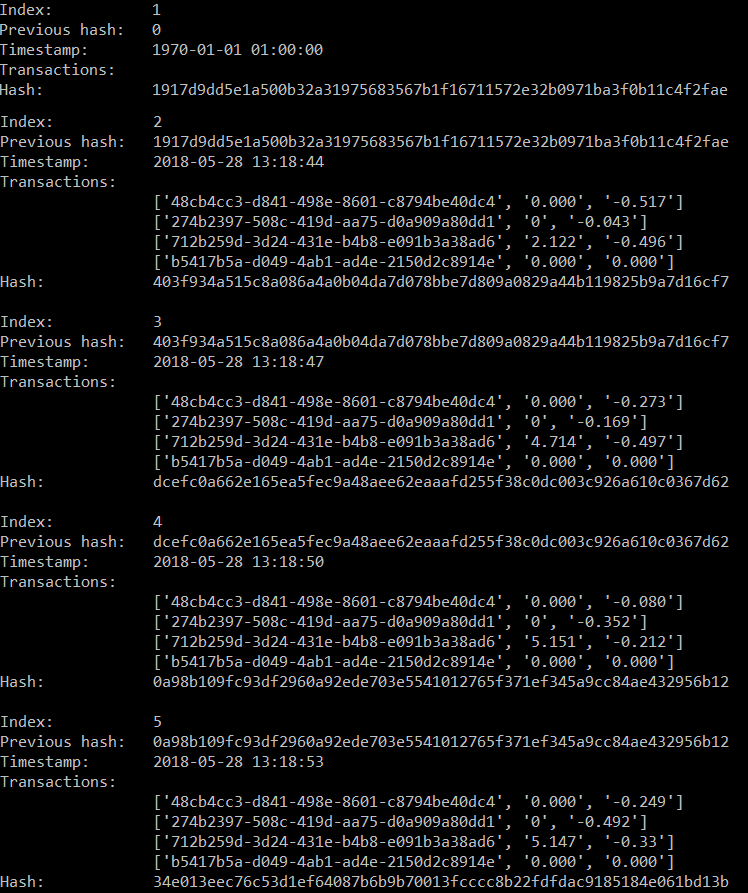
\includegraphics[width=1\linewidth]{Images/tx_1}
\end{subfigure}
\end{figure}
\begin{figure}\ContinuedFloat
\begin{subfigure}[b]{1\textwidth}
  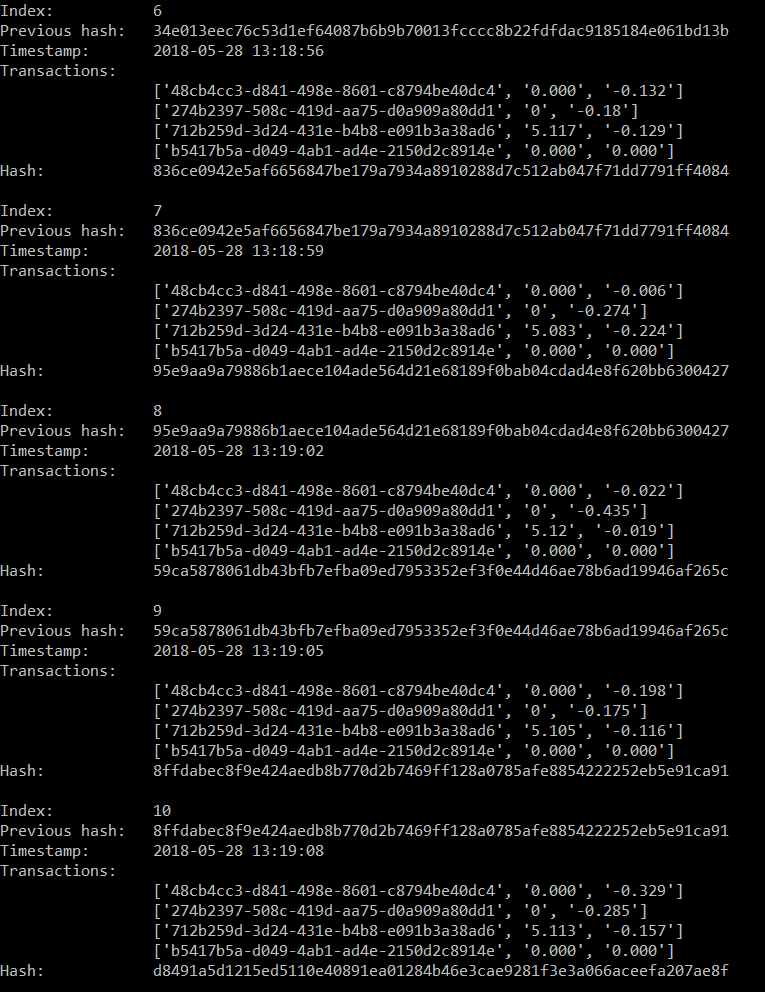
\includegraphics[width=1\linewidth]{Images/tx_2}
\end{subfigure}
\caption{10 first blocks in the blockchain.}
\label{fig:chain}
\end{figure}

\begin{figure}
\centering
\begin{subfigure}[!htb]{1\textwidth}
  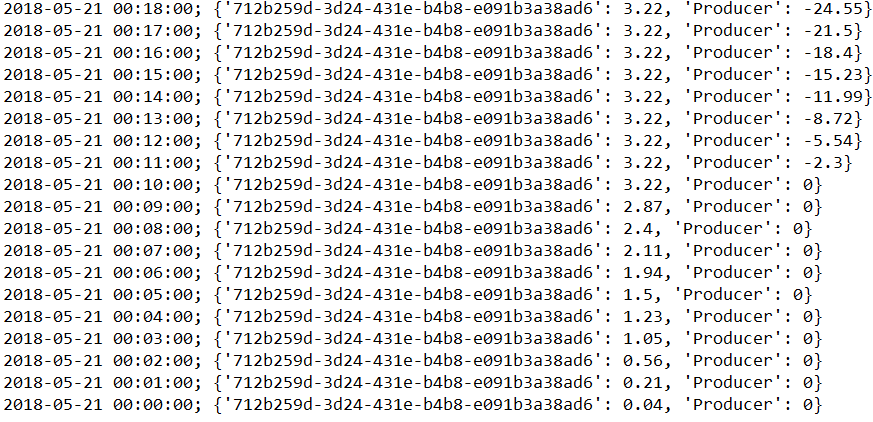
\includegraphics[width=1\linewidth]{Images/settle_2}
  \caption{Settlement for node 274b2397-508c-419d-aa75-d0a909a80dd1}
\end{subfigure}
\begin{subfigure}[b]{1\textwidth}
  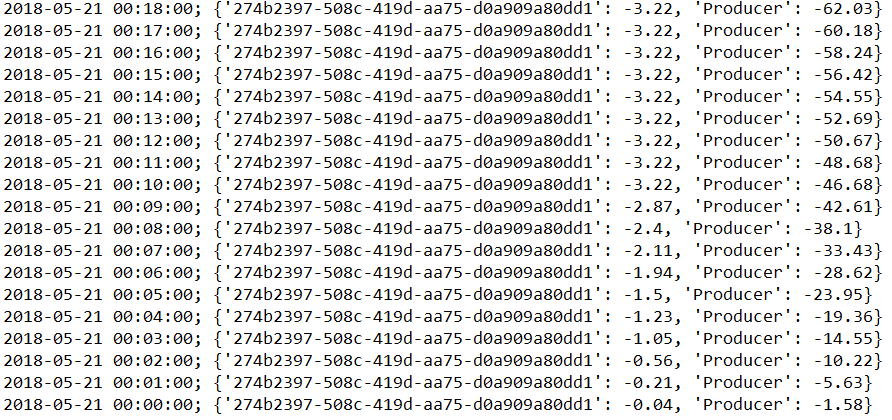
\includegraphics[width=1\linewidth]{Images/settle_7}
  \caption{Settlement for node 712b259d-3d24-431e-b4b8-e091b3a38ad6}
\end{subfigure}
\caption{Settlement between two prosumer nodes that have initiated a smart contract.}
\label{fig:settlement}
\end{figure}

Figure \ref{fig:settlement} shows the settlement between two of the nodes in the network. Each line represents the settlement of one transaction, with the most recent settlement at the top. Negative numbers represent money that is owned to the specified node, by the node who's settlement account is shown. Positive numbers represent money that the specified node owes the node who's settlement account is shown.

The results in figure \ref{fig:settlement} show thatnode 712b259d-3d24-431e-b4b8-e091b3a38ad6, the buyer, owes node 274b2397-508c-419d-aa75-d0a909a80dd1, the seller, 3.22 NOK after 19 minutes. Both nodes have consumed a considerable amount of electricity generated from the pure producers.

\section{Module Results}

\subsection{User Interface}
The results from the tests run on the user interface can be seen here. Figure \ref{monitor} shows how the consumption and production of electricity can be viewed in real-time for each node. Figure \ref{contract} show how the producers can  advertise their available excess electricity, and an approach for creating smart contracts from the buyers point of view.

\begin{figure}
\centering
\begin{subfigure}[!htb]{1\textwidth}
   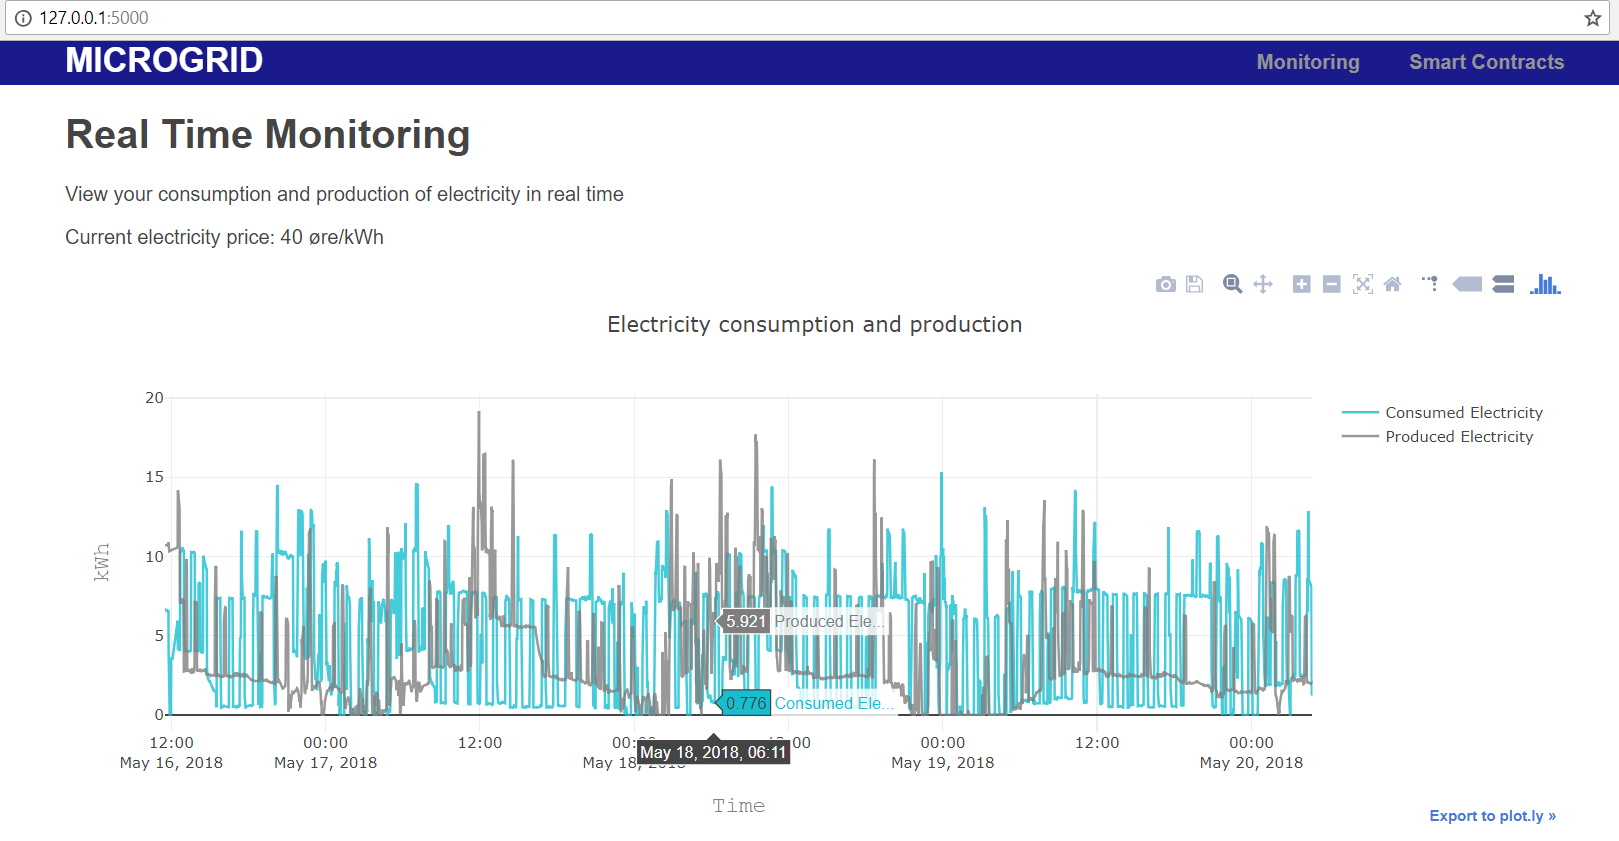
\includegraphics[width=1\linewidth]{Images/Monitor}
   \caption{}
   \label{fig:Ng1} 
\end{subfigure}

\begin{subfigure}[b]{1\textwidth}
   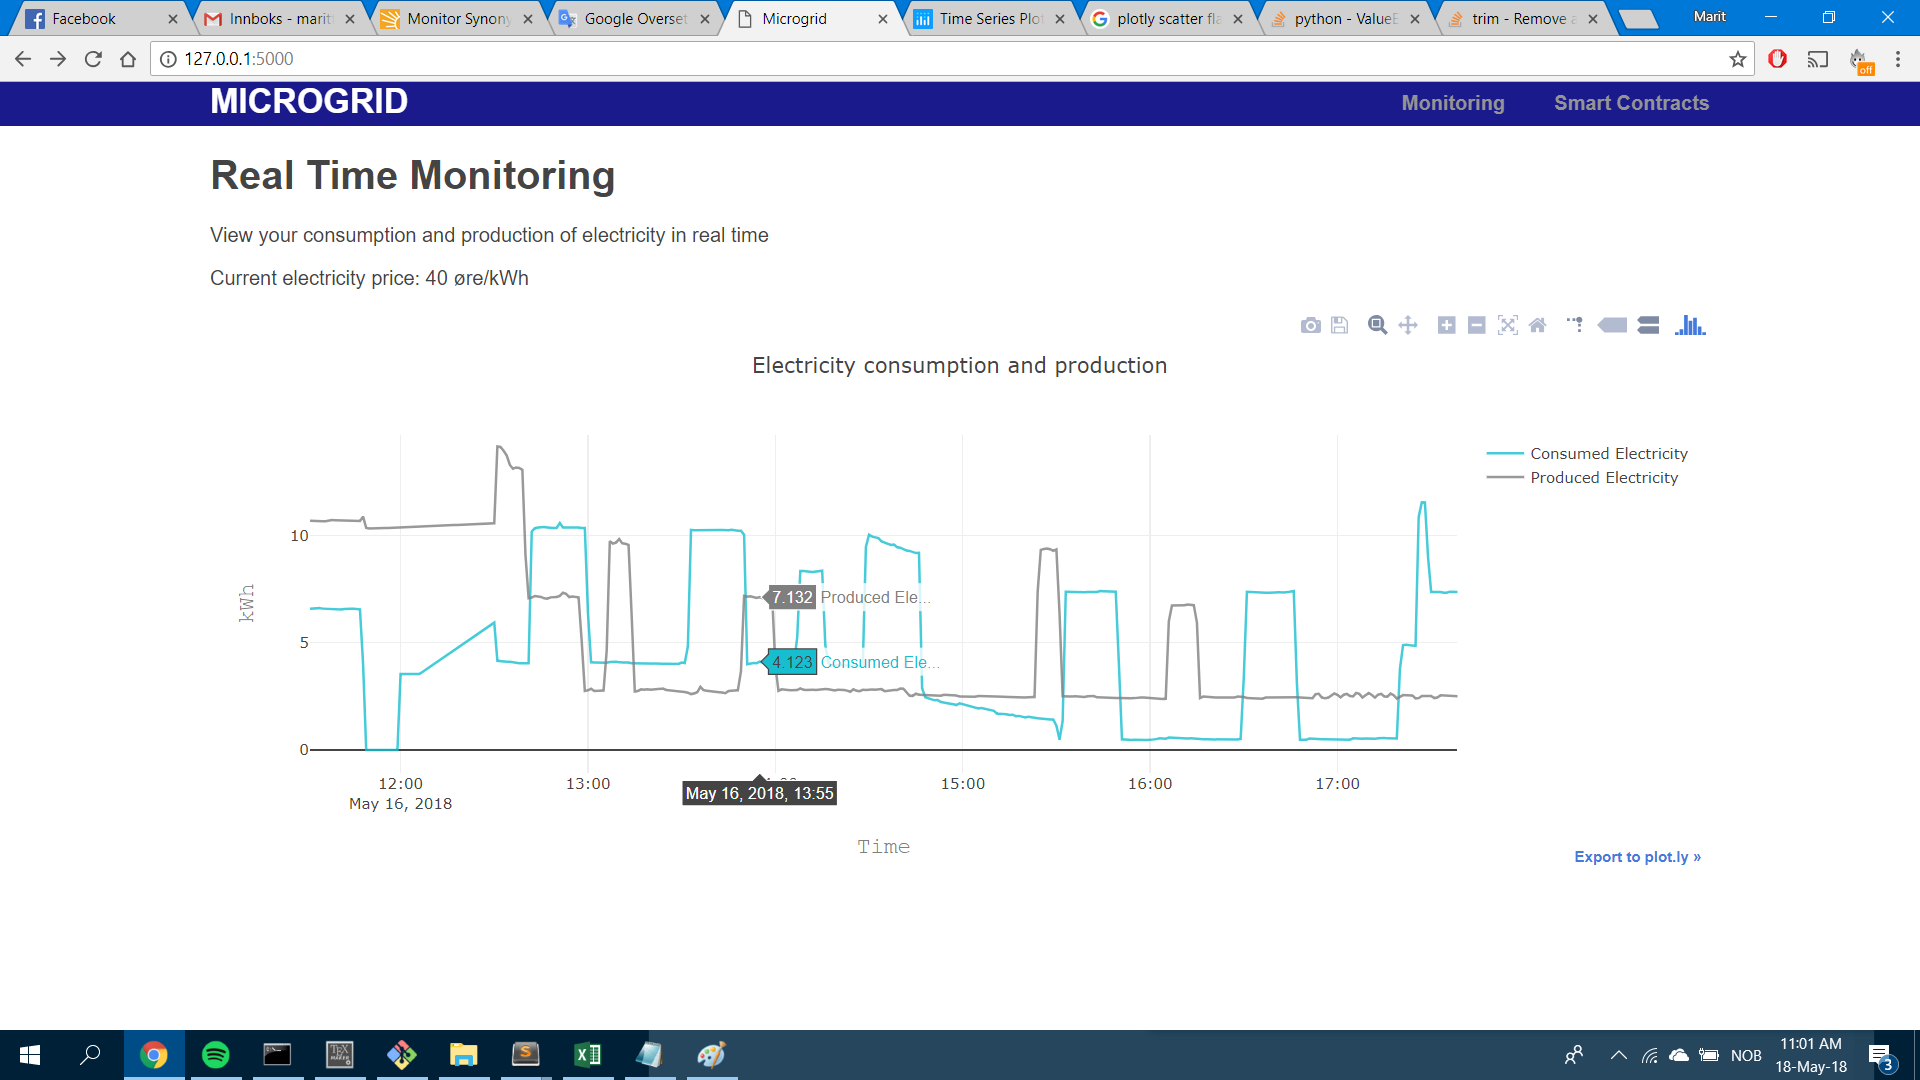
\includegraphics[width=1\linewidth]{Images/Monitor_zoomed}
   \caption{}
   \label{fig:Ng2}
\end{subfigure}

\caption{Real-time monitoring of consumed and produced electricity displayed on user interface. (a) shows the whole timeline and (b) shows a zoomed extract.}
\label{monitor}
\end{figure}


\begin{figure}[!htb]
\centering
	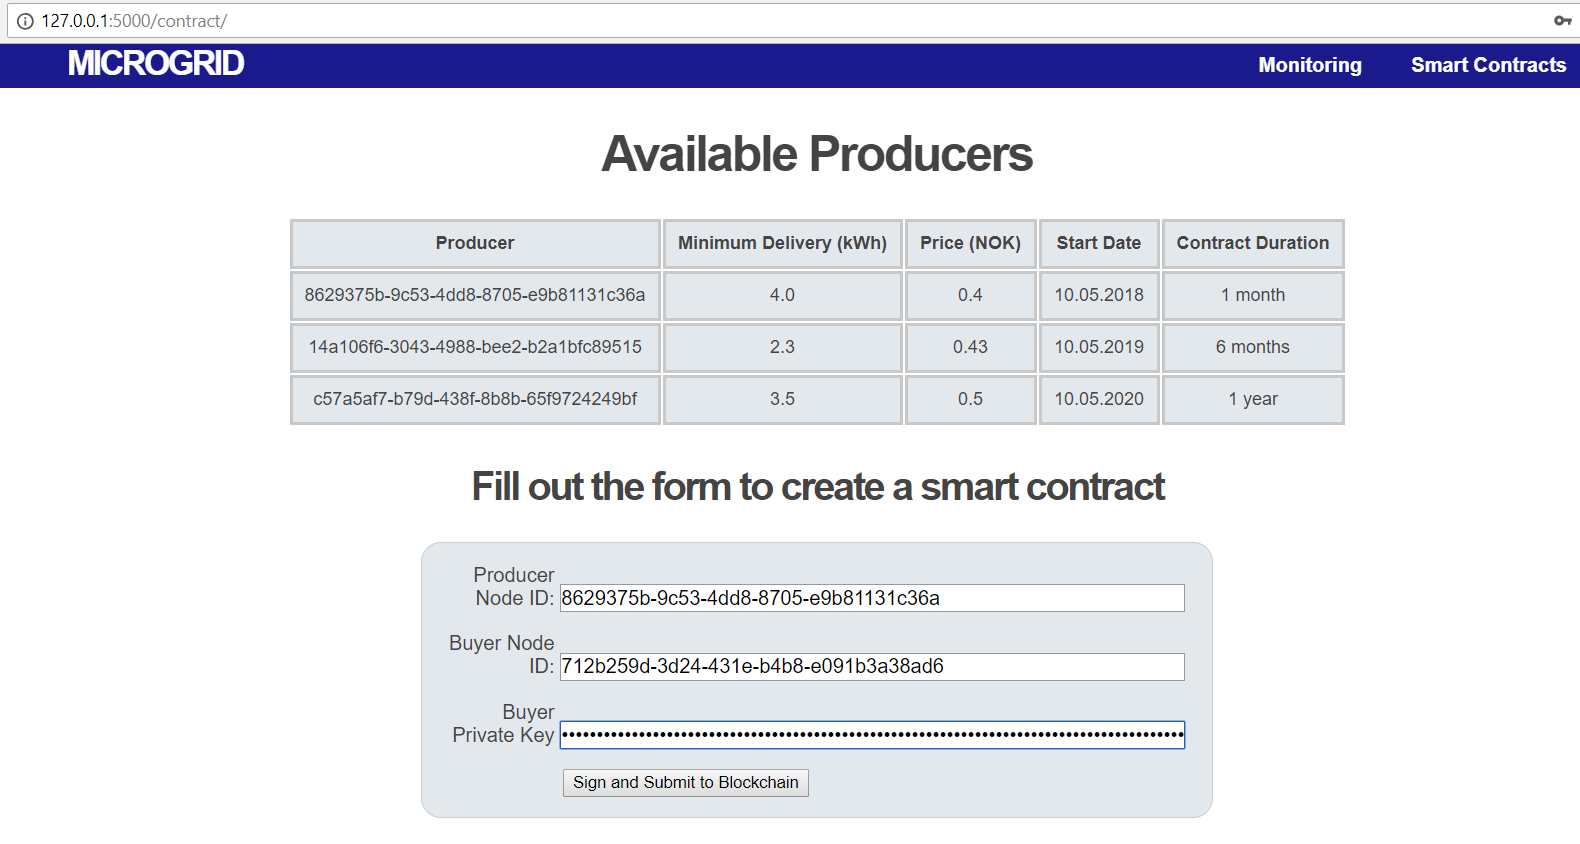
\includegraphics[width=1\textwidth]{Images/contract}
	\caption{Availability producers selling excess electricity.}
	\label{contract}
\end{figure}


\subsection{Unittests}

\subsection{Network Module}

\begin{figure}[!htb]
\centering
	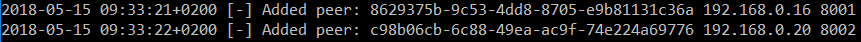
\includegraphics[width=1\textwidth]{Images/connection}
	\caption{Network communication between two computers on the same network.}
	\label{connection}
\end{figure}

Success for two machines on same network


Fail for two machines on different network, due to port forwarding issues

\subsection{Consensus}

\subsection{Smart Contract}\label{scres}
Image of signing/validation 